\documentclass[aspectratio=43,t]{beamer}
%\documentclass[aspectratio=169,t]{beamer}
%\documentclass[aspectratio=43,t,handout]{beamer}

\usepackage[utf8]{inputenc}
\usepackage[T1]{fontenc}
% English
\usepackage[english]{babel}
% or German?
%\usepackage[ngerman]{babel}
\usepackage{amsmath,amssymb}
\usepackage{graphicx}
\usepackage{listings}
\usepackage{csquotes}
\usepackage{tikz}

\usepackage[backend=bibtex,sorting=none,doi=false,style=phys]{biblatex}
\bibliography{./references}

% --------------------------------------------------------------------------------------------------------------------------------------------------------------------------
% THEME SETTINGS

%%%%%%%%%DO NOT REMOVE%%%%%%%%%%%
\makeatletter
\def\beamer@calltheme#1#2#3{\def\beamer@themelist{#2}
    \@for\beamer@themename:=\beamer@themelist\do
    {\usepackage[{#1}]{\beamer@themelocation/#3\beamer@themename}}}
\def\usefolder#1{\def\beamer@themelocation{#1}}
\def\beamer@themelocation{}
\usefolder{theme}

% Themes:
%  - fau:          FAU theme
%  - fau-tf:       TechFak FAU theme
%  - fau-tf-lme:   TechFak LME FAU theme
%
% Options:
%  - image:        Cover image on title page
%  - plain:        Plain title page
%  - longtitle:    Title page layout for long title
\usetheme[longtitle]{fau-tf-lme}

% END of THEME SETTINGS
% --------------------------------------------------------------------------------------------------------------------------------------------------------------------------

% Enable semi-transparent animation preview
\setbeamercovered{transparent}


\lstset{%
  language=C++,
  tabsize=2,
  basicstyle=\tt\scriptsize,
  keywordstyle=\color{blue},
  commentstyle=\color{green!50!black},
  stringstyle=\color{red},
  numbers=left,
  numbersep=0.5em,
  numberstyle=\tt\tiny
}

% --------------------------------------------------------------------------------------------------------------------------------------------------------------------------

% Title, authors, and date
\setbeamerfont{title}{size=\Large}
\title[CID]{Detection of Hand Drawn Electrical Circuit Diagrams and their Components using Deep Learning Methods and Conversion into LTspice Format}
\setbeamerfont{subtitle}{size=\large}
\subtitle{Final Talk: Dmitrij Vinokour}
\author[D.\ Vinokour]{Supervised by Florian Thamm M. Sc., Felix Denzinger M. Sc., Prof. Dr. Andreas Maier}
% English version
\institute[Pattern Recognition Lab]{Pattern Recognition Lab, Friedrich-Alexander University Erlangen-Nürnberg}
% German version
%\institute[Pattern Recognition Lab]{Image Fusion Group, Pattern Recognition Lab, Friedrich-Alexander-Universität Erlangen-Nürnberg}
\date{\today}


% Set additional partners logo in the headline for title and body pages
%Comment out this macro if no partner logo is needed.
% \setPartnerLogo{theme/art/tf/lme/partner-logo} % <-----  PARTNER LOGO

% Set additional seal or conference logo on the left side of the title page only. Does not overwrite the FAU seal!
%Comment out this macro if no conference logo is needed.
% \setLeftSeal{theme/art/tf/lme/conference-logo} % <-----  CONFERENCE LOGO


\begin{document}
  % Title
  \maketitle


{ % Motivation
\setbeamertemplate{footline}{}
\begin{frame}[noframenumbering]{Motivation}
%   Some motivational example\dots



  \fullcite{goossens93}
\end{frame}
}

{ % Outline
\setbeamertemplate{footline}{}
\begin{frame}[noframenumbering]{Outline}
  \tableofcontents
\end{frame}
}

\section{Introduction}



\subsection{Problem Statement}

\subsection{Related Work}

\section{Data}

\begin{block}{Data}

\begin{itemize}
    \item Collection of electrical circuit diagrams (ECDs) in German notation
    \item 31 Persons (21 train / valid, 10 test)
    \item Average 7.6 circuits / person
    \item Labeled with bounding boxes and segmentation masks
\end{itemize}

\begin{table}
\begin{center}
\footnotesize
\begin{tabular}{l|l|l|l|l|l|l}
    & \textbf{Images} & \textbf{Background} & \textbf{Annotated}  & \textbf{train ratio} & \textbf{valid ratio} & \textbf{test ratio}\\
    \hline
    & 110 & white & & 74.66\% & 6.69\% & 18.65\% \\
    & 17 & checkered & & 17.64\% & 11.77\% & 70.59\%\\
    & 89 & white & \checkmark & 78.65\% & 11.24\% & 10.11\%\\
    & 21 & checkered & \checkmark & 9.52\% & 19.05\% & 71.43\%\\
    \hline
    \textbf{Total} & 239 & & &45.12\% & 12.19\% & 42.69\%\\

\end{tabular}
\caption{General Overview Data}
\label{tab:data_overview}
\end{center}
\end{table}

% \begin{figure}
% \begin{center}
%     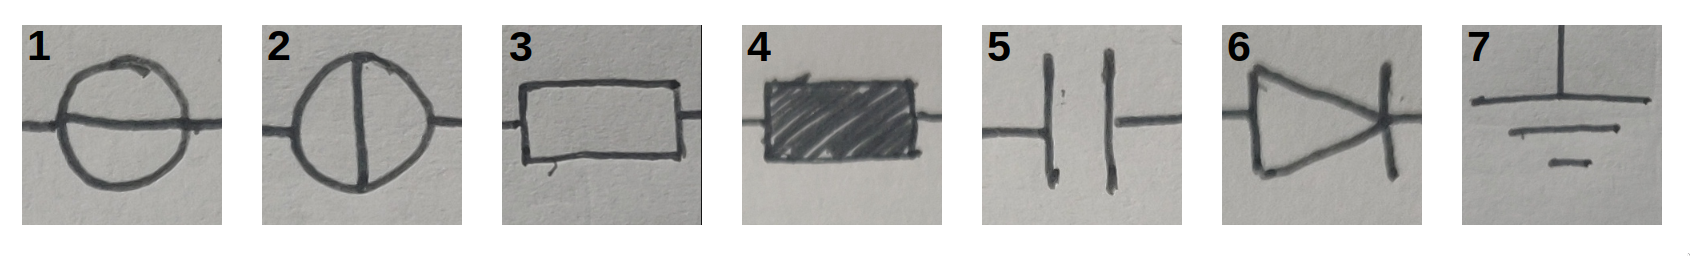
\includegraphics[width=8cm]{imgs/all.png}
%     \caption{Used electrical circuit components in German notation.}
%     \label{fig:used_eccs}
% \end{center}
% \end{figure}

\end{block}

\begin{frame}

\begin{table}
\begin{center}
\scriptsize
\begin{tabular}{l|l|l|l|l|}

\textbf{class} & \textbf{total} & \textbf{train ratio} & \textbf{valid ratio} & \textbf{test ratio} \\
    \hline
    diode left              & 156    &  83.33\%  &    8.97\%  &  7.69\% \\
    diode top               & 210    &  82.38\%  &    6.19\%  & 11.43\% \\
    diode right             & 150    &  82.00\%  &   12.67\%  &  5.33\% \\
    diode bottom            & 102    &  67.65\%  &   15.69\%  & 16.67\% \\
    resistor horizontal     & 318    &  71.38\%  &    6.92\%  & 21.70\% \\
    resistor vertical       & 350    &  66.00\%  &    6.57\%  & 27.43\% \\
    capacitor horizontal    & 405    &  85.68\%  &    4.94\%  &  9.38\% \\
    capacitor vertical      & 268    &  65.30\%  &   10.45\%  & 24.25\% \\
    ground left             & 137    &  72.99\%  &   10.95\%  & 16.06\% \\
    ground top              & 137    &  81.02\%  &   13.87\%  &  5.11\% \\
    ground right            & 116    &  78.45\%  &   14.66\%  &  6.90\% \\
    ground bottom           & 178    &  73.60\%  &   14.04\%  & 12.36\% \\
    inductor horizontal     & 251    &  76.89\%  &    8.37\%  & 14.74\% \\
    inductor vertical       & 290    &  73.45\%  &    9.31\%  & 17.24\% \\
    source horizontal       & 188    &  77.66\%  &   11.17\%  & 11.17\% \\
    source vertical         & 238    &  64.71\%  &   14.29\%  & 21.01\% \\
    current horizontal      & 202    &  77.72\%  &    9.41\%  & 12.87\% \\
    current vertical        & 220    &  75.00\%  &   12.73\%  & 12.27\% \\
    text                    & 877    &  61.92\%  &   16.76\%  & 21.32\% \\
    arrow left              & 57     &  70.18\%  &   19.30\%  & 10.53\% \\
    arrow top               & 77     &  64.94\%  &   23.38\%  & 11.69\% \\
    arrow right             & 105    &  70.48\%  &   16.19\%  & 13.33\% \\
    arrow bot               & 104    &  71.15\%  &   15.38\%  & 13.46\% \\
    \hline
    \textbf{total}          & 5136   &  73.65\%  &   12.27\%  & 14.08\% \\
\end{tabular}
\caption{Classwise Listed Data}
\label{tab:yolo_classes}
\end{center}
\end{table}

\end{frame}

\subsection{Pipeline}

\section{Training and Experiments}

\subsection{YOLOv4-Tiny}

\subsection{MobileNetV2-UNet}

% Body
\section{Lists}
\begin{frame}{Lists}
\begin{block}{List of Items}
  \begin{itemize}
    \item one
    \item two
    \item three
    \item \dots
  \end{itemize}
\end{block}

\pause

\begin{block}{Numbered List of Items}
  \begin{enumerate}
    \item<2-> one
    \item<3-> two
    \item<4-> three
    \item<5-> \dots
  \end{enumerate}
\end{block}
\end{frame}

\section{Listings}
\begin{frame}[fragile]{Listings}
\begin{lstlisting}[language=C++]
#include <iostream>

int main() {
  std::cout << "Hello World!" << std::endl;
  return 0;
}
\end{lstlisting}
\end{frame}

% ----------------------------------------
% THANK YOU SLIDE
% ----------------------------------------
\begin{frame}{Thank you for your attention.}
	\centering
	\vspace{1cm}

	\textbf{\large Questions?}

	\vspace{0.5cm}

	\begin{center}
		
\includegraphics[height=3.5cm]{./theme/art/tf/lme/qr-lme}

		\url{www5.cs.fau.de/~yourLastName}
	\end{center}
\end{frame}
\end{document}
